\documentclass{article}
\usepackage[preprint]{neurips_2024}
\usepackage[utf8]{inputenc}
\usepackage[T1]{fontenc}
\usepackage[colorlinks=true,linkcolor=black,citecolor=blue!50!black,urlcolor=blue!50!black]{hyperref}
\usepackage{url}
\usepackage{booktabs}
\usepackage{amsmath,amssymb,amsthm}
\usepackage{cancel}
\usepackage{microtype}
\usepackage{xcolor}
\usepackage{tikz}
\usetikzlibrary{arrows.meta,positioning}

\newtheorem{proposition}{Proposition}[section]
\newtheorem{lemma}[proposition]{Lemma}
\newtheorem{corollary}[proposition]{Corollary}
\theoremstyle{definition}
\newtheorem{definition}[proposition]{Definition}
\newtheorem{assumption}{Assumption}
\theoremstyle{remark}
\newtheorem{remark}[proposition]{Remark}

\newcommand{\E}{\mathbb{E}}
\newcommand{\dE}{\Delta E}
\newcommand{\dP}{\Delta P}
\newcommand{\Ob}{\bar O}
\newcommand{\KL}{\mathrm{KL}}
\newcommand{\why}[1]{\tag*{\small(#1)}}

\title{The State Defect, Empowerment and Plasticity}

\author{XXX}

\begin{document}
\maketitle

\begin{abstract}
For an agent that acts on a memory, we derive the empowerment and plasticity mismatches between the history and the memory, the two splits of the state defect, and three ways to separate the reward inside them. We then follow the defects $D_t,D_{t+1},D_{t+2},\dots$ of successive steps, write each term as an average log ratio of two predictions, show how the reward of each step enters the return over a few steps, and relate the return to the Bellman equation with the history and with the memory as the state. Every derivation is written term by term, and every cancellation names the assumption or lemma that allows it.
\end{abstract}

\section{Setting}\label{sec:setting}

\begin{center}
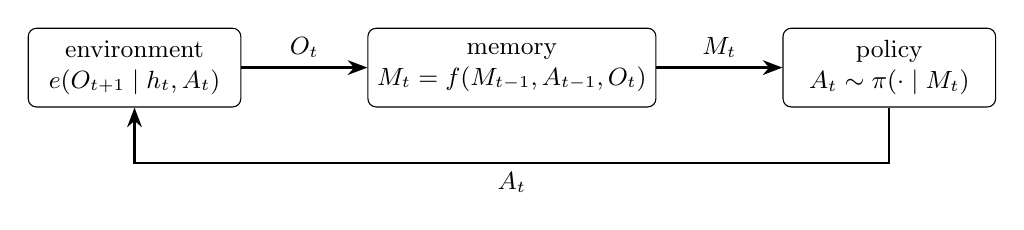
\begin{tikzpicture}[>={Stealth[length=2.5mm]}, node distance=10mm and 16mm,
  box/.style={draw, rounded corners=3pt, minimum height=10mm, minimum width=27mm, align=center, font=\small}]
\node[box] (world) {environment\\ $e(O_{t+1}\mid h_t, A_t)$};
\node[box, right=of world] (mem) {memory\\ $M_t = f(M_{t-1}, A_{t-1}, O_t)$};
\node[box, right=of mem] (pol) {policy\\ $A_t \sim \pi(\cdot \mid M_t)$};
\draw[->, thick] (world) -- node[above, font=\small] {$O_t$} (mem);
\draw[->, thick] (mem) -- node[above, font=\small] {$M_t$} (pol);
\draw[->, thick] (pol.south) -- ++(0,-7mm) -| node[pos=0.25, below, font=\small] {$A_t$} (world.south);
\end{tikzpicture}
\end{center}

The history is $h_t=(O_1,A_1,\dots,A_{t-1},O_t)$. The observation contains the reward: $O_t=(R_t,\Ob_t)$, with $\Ob_t$ the rest of the observation. All observation and action sets are finite, and all probabilities are under the law of the agent's experience induced by the three boxes.

\begin{assumption}[Environment]\label{as:env}
$O_{t+1}\sim e(\cdot\mid h_t,A_t)$ for some law $e$; the environment may depend on the whole history, with no Markov or stationarity condition.
\end{assumption}

\begin{assumption}[Memory]\label{as:mem}
$M_1=f_1(O_1)$ and $M_{t+1}=f(M_t,A_t,O_{t+1})$ for fixed maps $f_1,f$. Hence $M_t$ is a function of $h_t$.
\end{assumption}

\begin{assumption}[Policy]\label{as:pol}
$P(A_t=a\mid h_t)=\pi(a\mid M_t)$: the action depends on the history only through the memory.
\end{assumption}

Every identity in this note was checked numerically. The script \texttt{checks/verify\_note.py} computes the exact law of all trajectories in small random environments whose next observation depends on the whole history, and tests each numbered statement for a finite horizon; the largest error is $10^{-13}$.

\section{Tools}\label{sec:tools}

We use five standard facts \citep[Ch.~2]{cover2006elements}. $X,Y,W,Z$ are random variables, and conditioning on nothing is allowed.
\begin{enumerate}
\item[(T1)] $I(X;Y\mid Z)=H(X\mid Z)-H(X\mid Y,Z)=H(Y\mid Z)-H(Y\mid X,Z)$.
\item[(T2)] Chain rule: $I(X,Y;W\mid Z)=I(X;W\mid Z)+I(Y;W\mid Z,X)=I(Y;W\mid Z)+I(X;W\mid Z,Y)$, and the same with the pair in the second place, since $I$ is symmetric.
\item[(T3)] $I(X;Y\mid Z)\ge0$, with equality exactly when $X$ and $Y$ are independent given $Z$.
\item[(T4)] If $W$ is a function of $X$, conditioning on $(X,W)$ is the same as conditioning on $X$: $H(Y\mid X,W,Z)=H(Y\mid X,Z)$. By Assumption~\ref{as:mem}, this applies to $W=M_t$, $X=h_t$.
\item[(T5)] $h_{t+1}=(h_t,A_t,O_{t+1})$, so conditioning on $h_{t+1}$ is the same as conditioning on $(h_t,A_t,O_{t+1})$.
\end{enumerate}

\begin{lemma}[The action depends on the past only through the memory]\label{lem:action}
Under Assumptions~\ref{as:mem} and~\ref{as:pol}, for every $k\ge0$,
\[
H(A_{t+k}\mid h_t,A_t,O_{t+1},\dots,A_{t+k-1},O_{t+k})=H(A_{t+k}\mid M_t,A_t,O_{t+1},\dots,A_{t+k-1},O_{t+k}),
\]
and therefore $I(h_t;A_{t+k}\mid M_t,A_t,O_{t+1},\dots,A_{t+k-1},O_{t+k})=0$. The cases used most are
\begin{align*}
\text{(a) } k=0:&\quad H(A_t\mid h_t)=H(A_t\mid M_t),\\
\text{(b) } k=1:&\quad H(A_{t+1}\mid h_t,A_t,O_{t+1})=H(A_{t+1}\mid M_t,A_t,O_{t+1}).
\end{align*}
\end{lemma}

\begin{proof}
By (T5) applied $k$ times, the conditioning variables on the left are $h_{t+k}$. By Assumption~\ref{as:pol}, the law of $A_{t+k}$ given $h_{t+k}$ is $\pi(\cdot\mid M_{t+k})$. By Assumption~\ref{as:mem}, $M_{t+k}$ is obtained from $M_t$ by applying $f$ $k$ times with the inputs $(A_t,O_{t+1}),\dots,(A_{t+k-1},O_{t+k})$, so it is a function of the conditioning variables on the right. These variables are a function of $h_{t+k}$, so the law of $A_{t+k}$ given them is the average of $\pi(\cdot\mid M_{t+k})$ over the histories consistent with them, which is $\pi(\cdot\mid M_{t+k})$ itself. Both laws are $\pi(\cdot\mid M_{t+k})$, so the two entropies are equal. For the mutual information, write $C=(A_t,O_{t+1},\dots,A_{t+k-1},O_{t+k})$ in this proof only:
\begin{align*}
I(h_t;A_{t+k}\mid M_t,C)
&=H(A_{t+k}\mid M_t,C)-H(A_{t+k}\mid h_t,M_t,C) \why{T1}\\
&=H(A_{t+k}\mid M_t,C)-H(A_{t+k}\mid h_t,C) \why{T4}\\
&=0 \why{the equality of entropies above}.
\end{align*}
\end{proof}
\section{Empowerment and plasticity at the history and at the memory}\label{sec:EP}

In every derivation below, the label at the right of a line names the fact used to obtain that line. Two struck-through terms in a line are equal by the named fact and cancel.

\begin{definition}\label{def:EP}
Following the one-step form of \citet{abel2025plasticity}, the empowerment of the action and the plasticity of the next action, computed from the history and from the memory, are
\begin{align*}
E_t&=I(A_t;O_{t+1}\mid h_t), & E_t(M)&=I(A_t;O_{t+1}\mid M_t),\\
P_{t+1}&=I(O_{t+1};A_{t+1}\mid h_t,A_t), & P_{t+1}(M)&=I(O_{t+1};A_{t+1}\mid M_t,A_t),
\end{align*}
and the two mismatches are $\dE_t=E_t-E_t(M)$ and $\dP_t=P_{t+1}(M)-P_{t+1}$.
\end{definition}

\begin{proposition}[Empowerment mismatch]\label{prop:dE}
Under Assumptions~\ref{as:mem} and~\ref{as:pol}, $\dE_t=I(h_t;A_t\mid M_t,O_{t+1})\ge0$.
\end{proposition}

\begin{proof}
Write both empowerments with (T1), with $A_t$ as the variable whose entropy is taken:
\begin{align*}
E_t&=H(A_t\mid h_t)-H(A_t\mid h_t,O_{t+1}),\\
E_t(M)&=H(A_t\mid M_t)-H(A_t\mid M_t,O_{t+1}).
\end{align*}
Subtract:
\begin{align*}
\dE_t&=\cancel{H(A_t\mid h_t)}-H(A_t\mid h_t,O_{t+1})-\cancel{H(A_t\mid M_t)}+H(A_t\mid M_t,O_{t+1}) \why{struck terms equal, Lemma~\ref{lem:action}(a)}\\
&=H(A_t\mid M_t,O_{t+1})-H(A_t\mid h_t,O_{t+1})\\
&=H(A_t\mid M_t,O_{t+1})-H(A_t\mid h_t,M_t,O_{t+1}) \why{T4}\\
&=I(h_t;A_t\mid M_t,O_{t+1}) \why{T1},
\end{align*}
which is nonnegative by (T3).
\end{proof}

\begin{proposition}[Plasticity mismatch]\label{prop:dP}
Under Assumptions~\ref{as:mem} and~\ref{as:pol}, $\dP_t=I(h_t;A_{t+1}\mid M_t,A_t)\ge0$.
\end{proposition}

\begin{proof}
Write both plasticities with (T1), with $A_{t+1}$ as the variable whose entropy is taken:
\begin{align*}
P_{t+1}&=H(A_{t+1}\mid h_t,A_t)-H(A_{t+1}\mid h_t,A_t,O_{t+1}),\\
P_{t+1}(M)&=H(A_{t+1}\mid M_t,A_t)-H(A_{t+1}\mid M_t,A_t,O_{t+1}).
\end{align*}
Subtract:
\begin{align*}
\dP_t&=H(A_{t+1}\mid M_t,A_t)-\cancel{H(A_{t+1}\mid M_t,A_t,O_{t+1})}\\
&\quad-H(A_{t+1}\mid h_t,A_t)+\cancel{H(A_{t+1}\mid h_t,A_t,O_{t+1})} \why{struck terms equal, Lemma~\ref{lem:action}(b)}\\
&=H(A_{t+1}\mid M_t,A_t)-H(A_{t+1}\mid h_t,A_t)\\
&=H(A_{t+1}\mid M_t,A_t)-H(A_{t+1}\mid h_t,M_t,A_t) \why{T4}\\
&=I(h_t;A_{t+1}\mid M_t,A_t) \why{T1},
\end{align*}
which is nonnegative by (T3).
\end{proof}

In words: given the outcome, the history still tells something about the action that the memory does not, so the memory underestimates empowerment; and the history tells something about the next action that the memory does not, so the memory overestimates plasticity.

\section{The state defect and its two splits}\label{sec:splits}

\begin{definition}\label{def:terms}
The state defect and two further terms are
\[
D_t=I(h_t;O_{t+1}\mid M_t,A_t),\qquad D^0_t=I(h_t;O_{t+1}\mid M_t),\qquad D^+_t=I(h_t;O_{t+1}\mid M_t,A_t,A_{t+1}).
\]
With Propositions~\ref{prop:dE} and~\ref{prop:dP}, each of the five terms is a mutual information between the history and one variable, given the memory and other variables:
\begin{center}
\small
\begin{tabular}{llll}
\toprule
term & mutual information & variable predicted & given, besides $M_t$\\
\midrule
$D_t$ & $I(h_t;O_{t+1}\mid M_t,A_t)$ & $O_{t+1}$ & $A_t$\\
$D^0_t$ & $I(h_t;O_{t+1}\mid M_t)$ & $O_{t+1}$ & nothing\\
$\dE_t$ & $I(h_t;A_t\mid M_t,O_{t+1})$ & $A_t$ & $O_{t+1}$\\
$\dP_t$ & $I(h_t;A_{t+1}\mid M_t,A_t)$ & $A_{t+1}$ & $A_t$\\
$D^+_t$ & $I(h_t;O_{t+1}\mid M_t,A_t,A_{t+1})$ & $O_{t+1}$ & $A_t,A_{t+1}$\\
\bottomrule
\end{tabular}
\end{center}
By (T1) and (T4), each is the uncertainty about the predicted variable given the memory minus the uncertainty given the history.
\end{definition}

\begin{proposition}[First split]\label{prop:split1}
Under Assumptions~\ref{as:mem} and~\ref{as:pol}, $D_t=D^0_t+\dE_t$.
\end{proposition}

\begin{proof}
Apply (T2) to $I(h_t,A_t;O_{t+1}\mid M_t)$ in the two orders.

History first:
\begin{align*}
I(h_t,A_t;O_{t+1}\mid M_t)&=I(h_t;O_{t+1}\mid M_t)+I(A_t;O_{t+1}\mid M_t,h_t) \why{T2}\\
&=D^0_t+I(A_t;O_{t+1}\mid h_t) \why{Definition~\ref{def:terms}; T4}\\
&=D^0_t+E_t \why{Definition~\ref{def:EP}}.
\end{align*}
Action first:
\begin{align*}
I(h_t,A_t;O_{t+1}\mid M_t)&=I(A_t;O_{t+1}\mid M_t)+I(h_t;O_{t+1}\mid M_t,A_t) \why{T2}\\
&=E_t(M)+D_t \why{Definitions~\ref{def:EP} and~\ref{def:terms}}.
\end{align*}
The two right sides are equal, so $D^0_t+E_t=E_t(M)+D_t$, that is, $D_t=D^0_t+E_t-E_t(M)=D^0_t+\dE_t$.
\end{proof}

\begin{proposition}[Second split]\label{prop:split2}
Under Assumptions~\ref{as:mem} and~\ref{as:pol}, $D_t=\dP_t+D^+_t$.
\end{proposition}

\begin{proof}
Apply (T2) to $I(h_t;O_{t+1},A_{t+1}\mid M_t,A_t)$ in the two orders.

Next observation first:
\begin{align*}
I(h_t;O_{t+1},A_{t+1}\mid M_t,A_t)&=I(h_t;O_{t+1}\mid M_t,A_t)+I(h_t;A_{t+1}\mid M_t,A_t,O_{t+1}) \why{T2}\\
&=D_t+0 \why{Definition~\ref{def:terms}; Lemma~\ref{lem:action}, $k=1$}.
\end{align*}
Next action first:
\begin{align*}
I(h_t;O_{t+1},A_{t+1}\mid M_t,A_t)&=I(h_t;A_{t+1}\mid M_t,A_t)+I(h_t;O_{t+1}\mid M_t,A_t,A_{t+1}) \why{T2}\\
&=\dP_t+D^+_t \why{Proposition~\ref{prop:dP}; Definition~\ref{def:terms}}.
\end{align*}
The two right sides are equal.
\end{proof}

\begin{remark}[Both splits come from one quantity]\label{rem:orders}
Apply (T2) to $I(h_t;A_t,O_{t+1},A_{t+1}\mid M_t)$ in three orders. In the order of time, $(A_t,O_{t+1},A_{t+1})$, the terms are $I(h_t;A_t\mid M_t)=0$ (Lemma~\ref{lem:action}, $k=0$), $D_t$, and $I(h_t;A_{t+1}\mid M_t,A_t,O_{t+1})=0$ (Lemma~\ref{lem:action}, $k=1$). In the order $(O_{t+1},A_t,A_{t+1})$ they are $D^0_t$, $\dE_t$ and $I(h_t;A_{t+1}\mid M_t,O_{t+1},A_t)=0$. In the order $(A_t,A_{t+1},O_{t+1})$ they are $0$, $\dP_t$ and $D^+_t$. So the first split reads the action $A_t$ after the observation it produced, the second reads the next action $A_{t+1}$ before the observation it responds to, and in the order of time the two actions contribute nothing.
\end{remark}

\begin{corollary}\label{cor:consequences}
Under Assumptions~\ref{as:mem} and~\ref{as:pol}:
\begin{enumerate}
\item[(a)] $D_t=0$ if and only if $D^0_t=0$ and $\dE_t=0$, and if and only if $\dP_t=0$ and $D^+_t=0$;
\item[(b)] $\dP_t\le D_t$;
\item[(c)] $\dE_t\le H(A_t\mid M_t)$, so $\dE_t=0$ and $D_t=D^0_t$ when the policy is deterministic.
\end{enumerate}
\end{corollary}

\begin{proof}
(a) Each term is nonnegative (T3), and a sum of two nonnegative terms is zero exactly when both are. (b) From Proposition~\ref{prop:split2}, since $D^+_t\ge0$. (c) $\dE_t=H(A_t\mid M_t,O_{t+1})-H(A_t\mid h_t,O_{t+1})\le H(A_t\mid M_t,O_{t+1})\le H(A_t\mid M_t)$, where the first step drops a nonnegative entropy and the second uses that conditioning does not increase entropy, which is (T1) with (T3). A deterministic policy has $H(A_t\mid M_t)=0$; then Proposition~\ref{prop:split1} gives $D_t=D^0_t$.
\end{proof}

\section{Separating the reward}\label{sec:reward}

The observation is a pair, $O_{t+1}=(R_{t+1},\Ob_{t+1})$. We first split each term by a general pair $O_{t+1}=(X,Y)$, with $X$ taken first, and then consider three ways to separate the reward: reward first, $(X,Y)=(R_{t+1},\Ob_{t+1})$; rest first, $(X,Y)=(\Ob_{t+1},R_{t+1})$; and a partial information decomposition, which takes no order.

\subsection{A split by $O_{t+1}=(X,Y)$}

\begin{proposition}[$D_t$, $D^0_t$ and $D^+_t$]\label{prop:xy-D}
For $O_{t+1}=(X,Y)$,
\begin{align*}
D_t&=I(h_t;X\mid M_t,A_t)+I(h_t;Y\mid M_t,A_t,X),\\
D^0_t&=I(h_t;X\mid M_t)+I(h_t;Y\mid M_t,X),\\
D^+_t&=I(h_t;X\mid M_t,A_t,A_{t+1})+I(h_t;Y\mid M_t,A_t,A_{t+1},X),
\end{align*}
and every term on the right is nonnegative.
\end{proposition}

\begin{proof}
Each line is (T2) applied to $I(h_t;X,Y\mid\cdot)$ with $X$ first, and each term is nonnegative by (T3).
\end{proof}

\begin{proposition}[$\dE_t$]\label{prop:xy-E}
Under Assumptions~\ref{as:mem} and~\ref{as:pol}, for $O_{t+1}=(X,Y)$,
\[
\dE_t=\underbrace{\big[I(A_t;X\mid h_t)-I(A_t;X\mid M_t)\big]}_{X\text{ part}}+\underbrace{\big[I(A_t;Y\mid h_t,X)-I(A_t;Y\mid M_t,X)\big]}_{Y\text{ part}},
\]
where the $X$ part equals $I(h_t;A_t\mid M_t,X)\ge0$ and the $Y$ part can be negative.
\end{proposition}

\begin{proof}
By (T2), with $X$ first,
\begin{align*}
E_t&=I(A_t;X,Y\mid h_t)=I(A_t;X\mid h_t)+I(A_t;Y\mid h_t,X),\\
E_t(M)&=I(A_t;X,Y\mid M_t)=I(A_t;X\mid M_t)+I(A_t;Y\mid M_t,X).
\end{align*}
Subtracting and grouping the $X$ terms and the $Y$ terms gives the formula for $\dE_t=E_t-E_t(M)$. For the $X$ part, write both terms with (T1), with $A_t$ as the variable whose entropy is taken:
\begin{align*}
&I(A_t;X\mid h_t)-I(A_t;X\mid M_t)\\
&\quad=\cancel{H(A_t\mid h_t)}-H(A_t\mid h_t,X)-\cancel{H(A_t\mid M_t)}+H(A_t\mid M_t,X) \why{struck terms equal, Lemma~\ref{lem:action}(a)}\\
&\quad=H(A_t\mid M_t,X)-H(A_t\mid h_t,M_t,X) \why{T4}\\
&\quad=I(h_t;A_t\mid M_t,X) \why{T1}.
\end{align*}
The $Y$ part is a difference of two mutual informations with different conditioning, and no lemma relates them.
\end{proof}

\begin{proposition}[$\dP_t$]\label{prop:xy-P}
Under Assumptions~\ref{as:mem} and~\ref{as:pol}, for $O_{t+1}=(X,Y)$,
\[
\begin{aligned}
\dP_t&=\underbrace{\big[I(X;A_{t+1}\mid M_t,A_t)-I(X;A_{t+1}\mid h_t,A_t)\big]}_{X\text{ part}}\\
&\quad+\underbrace{\big[I(Y;A_{t+1}\mid M_t,A_t,X)-I(Y;A_{t+1}\mid h_t,A_t,X)\big]}_{Y\text{ part}},
\end{aligned}
\]
where the $Y$ part equals $I(h_t;A_{t+1}\mid M_t,A_t,X)\ge0$ and the $X$ part can be negative.
\end{proposition}

\begin{proof}
By (T2), with $X$ first,
\begin{align*}
P_{t+1}&=I(X,Y;A_{t+1}\mid h_t,A_t)=I(X;A_{t+1}\mid h_t,A_t)+I(Y;A_{t+1}\mid h_t,A_t,X),\\
P_{t+1}(M)&=I(X,Y;A_{t+1}\mid M_t,A_t)=I(X;A_{t+1}\mid M_t,A_t)+I(Y;A_{t+1}\mid M_t,A_t,X).
\end{align*}
Subtracting gives the formula for $\dP_t=P_{t+1}(M)-P_{t+1}$. For the $Y$ part, write both terms with (T1), with $A_{t+1}$ as the variable whose entropy is taken, and use $(X,Y)=O_{t+1}$:
\begin{align*}
&I(Y;A_{t+1}\mid M_t,A_t,X)-I(Y;A_{t+1}\mid h_t,A_t,X)\\
&\quad=H(A_{t+1}\mid M_t,A_t,X)-\cancel{H(A_{t+1}\mid M_t,A_t,O_{t+1})}\\
&\qquad-H(A_{t+1}\mid h_t,A_t,X)+\cancel{H(A_{t+1}\mid h_t,A_t,O_{t+1})} \why{struck terms equal, Lemma~\ref{lem:action}(b)}\\
&\quad=H(A_{t+1}\mid M_t,A_t,X)-H(A_{t+1}\mid h_t,M_t,A_t,X) \why{T4}\\
&\quad=I(h_t;A_{t+1}\mid M_t,A_t,X) \why{T1}.
\end{align*}
The $X$ part is a difference of two mutual informations with different conditioning, and no lemma relates them.
\end{proof}

\begin{proposition}[The two splits for each part]\label{prop:xy-splits}
Under Assumptions~\ref{as:mem} and~\ref{as:pol}, for $O_{t+1}=(X,Y)$, the $X$ part and the $Y$ part of $D_t$ each split in the two ways of Section~\ref{sec:splits}:
\begin{align*}
I(h_t;X\mid M_t,A_t)&=I(h_t;X\mid M_t)+\big[I(A_t;X\mid h_t)-I(A_t;X\mid M_t)\big] \tag*{\small first split}\\
&=\big[I(X;A_{t+1}\mid M_t,A_t)-I(X;A_{t+1}\mid h_t,A_t)\big]+I(h_t;X\mid M_t,A_t,A_{t+1}) \tag*{\small second split},\\[4pt]
I(h_t;Y\mid M_t,A_t,X)&=I(h_t;Y\mid M_t,X)+\big[I(A_t;Y\mid h_t,X)-I(A_t;Y\mid M_t,X)\big] \tag*{\small first split}\\
&=I(h_t;A_{t+1}\mid M_t,A_t,X)+I(h_t;Y\mid M_t,A_t,A_{t+1},X) \tag*{\small second split}.
\end{align*}
So each part of $D_t$ is the sum of the same part of $D^0_t$ and of $\dE_t$, and of the same part of $\dP_t$ and of $D^+_t$.
\end{proposition}

\begin{proof}
\emph{$X$ part, first split.} Apply (T2) to $I(h_t,A_t;X\mid M_t)$ in two orders:
\begin{align*}
I(h_t,A_t;X\mid M_t)&=I(h_t;X\mid M_t)+I(A_t;X\mid M_t,h_t)=I(h_t;X\mid M_t)+I(A_t;X\mid h_t) \why{T2; T4}\\
&=I(A_t;X\mid M_t)+I(h_t;X\mid M_t,A_t) \why{T2}.
\end{align*}
Equate the two lines and solve for $I(h_t;X\mid M_t,A_t)$.

\emph{$X$ part, second split.} Write the $X$ part of $\dP_t$ with (T1), with $X$ as the variable whose entropy is taken, and regroup:
\begin{align*}
&I(X;A_{t+1}\mid M_t,A_t)-I(X;A_{t+1}\mid h_t,A_t)\\
&\quad=\big[H(X\mid M_t,A_t)-H(X\mid M_t,A_t,A_{t+1})\big]-\big[H(X\mid h_t,A_t)-H(X\mid h_t,A_t,A_{t+1})\big] \why{T1}\\
&\quad=\big[H(X\mid M_t,A_t)-H(X\mid h_t,A_t)\big]-\big[H(X\mid M_t,A_t,A_{t+1})-H(X\mid h_t,A_t,A_{t+1})\big] \why{regroup}\\
&\quad=I(h_t;X\mid M_t,A_t)-I(h_t;X\mid M_t,A_t,A_{t+1}) \why{T4; T1}.
\end{align*}
Move the last term to the left side.

\emph{$Y$ part, first split.} Apply (T2) to $I(h_t,A_t;Y\mid M_t,X)$ in two orders:
\begin{align*}
I(h_t,A_t;Y\mid M_t,X)&=I(h_t;Y\mid M_t,X)+I(A_t;Y\mid h_t,X) \why{T2; T4}\\
&=I(A_t;Y\mid M_t,X)+I(h_t;Y\mid M_t,A_t,X) \why{T2}.
\end{align*}
Equate and solve for $I(h_t;Y\mid M_t,A_t,X)$.

\emph{$Y$ part, second split.} Apply (T2) to $I(h_t;Y,A_{t+1}\mid M_t,A_t,X)$ in two orders:
\begin{align*}
I(h_t;Y,A_{t+1}\mid M_t,A_t,X)&=I(h_t;Y\mid M_t,A_t,X)+I(h_t;A_{t+1}\mid M_t,A_t,X,Y) \why{T2}\\
&=I(h_t;Y\mid M_t,A_t,X)+0 \why{$(X,Y)=O_{t+1}$; Lemma~\ref{lem:action}, $k=1$}\\
I(h_t;Y,A_{t+1}\mid M_t,A_t,X)&=I(h_t;A_{t+1}\mid M_t,A_t,X)+I(h_t;Y\mid M_t,A_t,A_{t+1},X) \why{T2}.
\end{align*}
Equate the two.
\end{proof}

So, whichever part comes first, its empowerment part is nonnegative and its plasticity part is signed; for the part that comes second, it is the other way round.

\subsection{Reward first and rest first}

Propositions~\ref{prop:xy-D}--\ref{prop:xy-P} with the two choices of $(X,Y)$ give the following. In every line, the term on the left is the sum of its reward part and its rest part. Every term written as a single mutual information is nonnegative; the terms in brackets can be negative.

\paragraph{Reward first,} $(X,Y)=(R_{t+1},\Ob_{t+1})$: the reward part comes first in each line.
\begin{align*}
D_t&=I(h_t;R_{t+1}\mid M_t,A_t)+I(h_t;\Ob_{t+1}\mid M_t,A_t,R_{t+1}),\\
D^0_t&=I(h_t;R_{t+1}\mid M_t)+I(h_t;\Ob_{t+1}\mid M_t,R_{t+1}),\\
D^+_t&=I(h_t;R_{t+1}\mid M_t,A_t,A_{t+1})+I(h_t;\Ob_{t+1}\mid M_t,A_t,A_{t+1},R_{t+1}),\\
\dE_t&=I(h_t;A_t\mid M_t,R_{t+1})+\big[I(A_t;\Ob_{t+1}\mid h_t,R_{t+1})-I(A_t;\Ob_{t+1}\mid M_t,R_{t+1})\big],\\
\dP_t&=\big[I(R_{t+1};A_{t+1}\mid M_t,A_t)-I(R_{t+1};A_{t+1}\mid h_t,A_t)\big]+I(h_t;A_{t+1}\mid M_t,A_t,R_{t+1}).
\end{align*}

\paragraph{Rest first,} $(X,Y)=(\Ob_{t+1},R_{t+1})$: the reward part comes second in each line.
\begin{align*}
D_t&=I(h_t;\Ob_{t+1}\mid M_t,A_t)+I(h_t;R_{t+1}\mid M_t,A_t,\Ob_{t+1}),\\
D^0_t&=I(h_t;\Ob_{t+1}\mid M_t)+I(h_t;R_{t+1}\mid M_t,\Ob_{t+1}),\\
D^+_t&=I(h_t;\Ob_{t+1}\mid M_t,A_t,A_{t+1})+I(h_t;R_{t+1}\mid M_t,A_t,A_{t+1},\Ob_{t+1}),\\
\dE_t&=I(h_t;A_t\mid M_t,\Ob_{t+1})+\big[I(A_t;R_{t+1}\mid h_t,\Ob_{t+1})-I(A_t;R_{t+1}\mid M_t,\Ob_{t+1})\big],\\
\dP_t&=\big[I(\Ob_{t+1};A_{t+1}\mid M_t,A_t)-I(\Ob_{t+1};A_{t+1}\mid h_t,A_t)\big]+I(h_t;A_{t+1}\mid M_t,A_t,\Ob_{t+1}).
\end{align*}
The co-information of $X,Y,W$ given $Z$ is $I(X;Y;W\mid Z)=I(X;Y\mid Z)-I(X;Y\mid Z,W)$. It is symmetric in $X,Y,W$, by (T2) applied to $I(X;Y,W\mid Z)$ in two orders, and it can be negative.

\begin{proposition}[How the two orders differ]\label{prop:orderdiff}
Under Assumptions~\ref{as:mem} and~\ref{as:pol}, the reward part in the reward-first order minus the reward part in the rest-first order is
\begin{align*}
\text{for }D_t:&\quad I(h_t;R_{t+1};\Ob_{t+1}\mid M_t,A_t),\\
\text{for }D^0_t:&\quad I(h_t;R_{t+1};\Ob_{t+1}\mid M_t),\\
\text{for }D^+_t:&\quad I(h_t;R_{t+1};\Ob_{t+1}\mid M_t,A_t,A_{t+1}),\\
\text{for }\dE_t:&\quad I(A_t;R_{t+1};\Ob_{t+1}\mid h_t)-I(A_t;R_{t+1};\Ob_{t+1}\mid M_t),\\
\text{for }\dP_t:&\quad I(R_{t+1};A_{t+1};\Ob_{t+1}\mid M_t,A_t)-I(R_{t+1};A_{t+1};\Ob_{t+1}\mid h_t,A_t).
\end{align*}
The rest parts differ by the same amounts with the opposite sign.
\end{proposition}

\begin{proof}
For $D_t$, the difference of the two reward parts above is $I(h_t;R_{t+1}\mid M_t,A_t)-I(h_t;R_{t+1}\mid M_t,A_t,\Ob_{t+1})$, which is the co-information by its definition; $D^0_t$ and $D^+_t$ are the same with other conditioning variables. For $\dE_t$, the reward part in the reward-first order is $I(A_t;R_{t+1}\mid h_t)-I(A_t;R_{t+1}\mid M_t)$ (Proposition~\ref{prop:xy-E}), and in the rest-first order it is $I(A_t;R_{t+1}\mid h_t,\Ob_{t+1})-I(A_t;R_{t+1}\mid M_t,\Ob_{t+1})$. Their difference is
\[
\big[I(A_t;R_{t+1}\mid h_t)-I(A_t;R_{t+1}\mid h_t,\Ob_{t+1})\big]-\big[I(A_t;R_{t+1}\mid M_t)-I(A_t;R_{t+1}\mid M_t,\Ob_{t+1})\big],
\]
and each bracket is a co-information by definition. The case of $\dP_t$ is the same with $I(R_{t+1};A_{t+1}\mid\cdot)$ in place of $I(A_t;R_{t+1}\mid\cdot)$, using Proposition~\ref{prop:xy-P}. The totals do not depend on the order, so the rest parts differ by the opposite amounts.
\end{proof}

\subsection{Without an order: four parts of $D_t$}

The two orders differ in where they put two kinds of information about the history: what the reward and the rest of the observation both carry, and what they carry only together. A partial information decomposition \citep{williams2010nonnegative} gives each kind its own part instead of assigning it to the reward or to the rest.

\begin{definition}[Four parts of $D_t$]\label{def:pid}
A split of $D_t$ into four parts is a choice of four nonnegative numbers:
\begin{itemize}
\item $D^{\mathrm{shared}}_t$, the information about the history, beyond the memory and the action, that the reward carries and the rest of the observation also carries;
\item $D^{R\,\mathrm{only}}_t$, the information that only the reward carries;
\item $D^{\Ob\,\mathrm{only}}_t$, the information that only the rest of the observation carries;
\item $D^{\mathrm{joint}}_t$, the information that the reward and the rest carry only together;
\end{itemize}
such that
\begin{align*}
I(h_t;R_{t+1}\mid M_t,A_t)&=D^{\mathrm{shared}}_t+D^{R\,\mathrm{only}}_t,\\
I(h_t;\Ob_{t+1}\mid M_t,A_t)&=D^{\mathrm{shared}}_t+D^{\Ob\,\mathrm{only}}_t,\\
D_t=I(h_t;R_{t+1},\Ob_{t+1}\mid M_t,A_t)&=D^{\mathrm{shared}}_t+D^{R\,\mathrm{only}}_t+D^{\Ob\,\mathrm{only}}_t+D^{\mathrm{joint}}_t.
\end{align*}
More precisely, the three equations are required for the conditional law given each value of $(M_t,A_t)$, and the four parts are the averages over these values \citep[Definition~3]{matthias2025novel}. The three equations leave one degree of freedom, which a choice of measure fixes. In the literature the four parts are called the redundant, the two unique, and the synergistic information.
\end{definition}

\begin{proposition}[The two orders in terms of the four parts]\label{prop:pid}
For any split of $D_t$ into four parts:
\begin{enumerate}
\item[(a)] the reward part of $D_t$ is $D^{\mathrm{shared}}_t+D^{R\,\mathrm{only}}_t$ in the reward-first order and $D^{R\,\mathrm{only}}_t+D^{\mathrm{joint}}_t$ in the rest-first order;
\item[(b)] their difference, the co-information of Proposition~\ref{prop:orderdiff}, is $I(h_t;R_{t+1};\Ob_{t+1}\mid M_t,A_t)=D^{\mathrm{shared}}_t-D^{\mathrm{joint}}_t$;
\item[(c)] the part that only the reward carries is bounded, whatever the measure, by
\begin{align*}
D^{R\,\mathrm{only}}_t&\ge\max\big(0,\ I(h_t;R_{t+1}\mid M_t,A_t)-I(h_t;\Ob_{t+1}\mid M_t,A_t)\big),\\
D^{R\,\mathrm{only}}_t&\le\min\big(I(h_t;R_{t+1}\mid M_t,A_t),\ I(h_t;R_{t+1}\mid M_t,A_t,\Ob_{t+1})\big).
\end{align*}
\end{enumerate}
\end{proposition}

\begin{proof}
Fix a value $(m,a)$ of $(M_t,A_t)$ and work with the conditional law given $(M_t,A_t)=(m,a)$; write the four parts at $(m,a)$ without the index $t$.

(a) The reward-first reward part is $I(h_t;R_{t+1}\mid m,a)$, which is $D^{\mathrm{shared}}+D^{R\,\mathrm{only}}$ by the first equation. The rest-first reward part is $I(h_t;R_{t+1}\mid m,a,\Ob_{t+1})$, and by (T2),
\begin{align*}
I(h_t;R_{t+1}\mid m,a,\Ob_{t+1})&=I(h_t;R_{t+1},\Ob_{t+1}\mid m,a)-I(h_t;\Ob_{t+1}\mid m,a) \why{T2}\\
&=\big(D^{\mathrm{shared}}+D^{R\,\mathrm{only}}+D^{\Ob\,\mathrm{only}}+D^{\mathrm{joint}}\big)-\big(D^{\mathrm{shared}}+D^{\Ob\,\mathrm{only}}\big) \why{third and second equations}\\
&=D^{R\,\mathrm{only}}+D^{\mathrm{joint}}.
\end{align*}

(b) Subtract the two results of (a): $(D^{\mathrm{shared}}+D^{R\,\mathrm{only}})-(D^{R\,\mathrm{only}}+D^{\mathrm{joint}})=D^{\mathrm{shared}}-D^{\mathrm{joint}}$. By Proposition~\ref{prop:orderdiff}, the same difference is the co-information.

(c) Subtracting the second equation from the first gives $D^{R\,\mathrm{only}}-D^{\Ob\,\mathrm{only}}=I(h_t;R_{t+1}\mid m,a)-I(h_t;\Ob_{t+1}\mid m,a)$; since $D^{\Ob\,\mathrm{only}}\ge0$, $D^{R\,\mathrm{only}}$ is at least the right side, and it is at least $0$. In (a), $D^{\mathrm{shared}}\ge0$ and $D^{\mathrm{joint}}\ge0$ give the two upper bounds.

Average over $(m,a)$. The identities are linear and hold for the averages. The upper bounds hold for the averages because the average of a minimum is at most the minimum of the averages, and the lower bound because the average of $\max(0,x_{m,a})$ is at least $\max(0,\text{average of }x_{m,a})$.
\end{proof}

So the reward-first order gives the reward the shared part, the rest-first order gives it the joint part, and the part that belongs to the reward in both orders is $D^{R\,\mathrm{only}}_t$. The difference between the orders, $D^{\mathrm{shared}}_t-D^{\mathrm{joint}}_t$, is positive when the shared part is larger and negative when the joint part is larger. With the measure of \citet{bertschinger2014quantifying}, $D^{R\,\mathrm{only}}_t>0$ exactly when there is a decision problem in which seeing the reward is strictly better than seeing the rest of the observation. The same split applies to $D^0_t$ and $D^+_t$ with other conditioning variables. The terms $\dE_t$ and $\dP_t$ involve an action as a third variable, and an order-free split of their reward parts would need a decomposition with three sources; we leave this open.

\section{From the defects at each step to the return}\label{sec:return}

\subsection{The terms at each step}

Sections~\ref{sec:splits} and~\ref{sec:reward} hold at every time. At the times $n=t,t+1,t+2$, the agent's own terms are
\begin{align*}
D_n&=D^0_n+\dE_n=\dP_n+D^+_n,\\
D_n&=I(h_n;R_{n+1}\mid M_n,A_n)+I(h_n;\Ob_{n+1}\mid M_n,A_n,R_{n+1}),\\
D^0_n&=I(h_n;R_{n+1}\mid M_n)+I(h_n;\Ob_{n+1}\mid M_n,R_{n+1}),\\
D^+_n&=I(h_n;R_{n+1}\mid M_n,A_n,A_{n+1})+I(h_n;\Ob_{n+1}\mid M_n,A_n,A_{n+1},R_{n+1}),\\
\dE_n&=I(h_n;A_n\mid M_n,R_{n+1})+\big[I(A_n;\Ob_{n+1}\mid h_n,R_{n+1})-I(A_n;\Ob_{n+1}\mid M_n,R_{n+1})\big],\\
\dP_n&=\big[I(R_{n+1};A_{n+1}\mid M_n,A_n)-I(R_{n+1};A_{n+1}\mid h_n,A_n)\big]+I(h_n;A_{n+1}\mid M_n,A_n,R_{n+1}),
\end{align*}
by Propositions~\ref{prop:split1} and~\ref{prop:split2} and the reward-first lines of Section~\ref{sec:reward}, with $n$ in place of $t$; in each of the last five lines the first term is the reward part and the second the rest part. The defect at time $n$ concerns the observation $O_{n+1}$, so the reward it contains is $R_{n+1}$:
\begin{center}
\small
\begin{tabular}{lll}
\toprule
time & defect & reward in its observation\\
\midrule
$t$ & $D_t$ & $R_{t+1}$\\
$t+1$ & $D_{t+1}$ & $R_{t+2}$\\
$t+2$ & $D_{t+2}$ & $R_{t+3}$\\
\bottomrule
\end{tabular}
\end{center}

\subsection{Each term as a ratio of two probabilities}

\begin{lemma}[Information as a ratio of predictions]\label{lem:ratio}
Under Assumption~\ref{as:mem}, for any variables $X$ and $Z$ and any time $n$,
\[
I(h_n;X\mid M_n,Z)=\E\Big[\log\frac{P(X\mid h_n,Z)}{P(X\mid M_n,Z)}\Big]=\E\Big[\KL\big(P(X\mid h_n,Z)\,\big\|\,P(X\mid M_n,Z)\big)\Big],
\]
and the memory's prediction is the average of the history's predictions over the histories behind the memory:
\[
P(X=x\mid M_n=m,Z=z)=\sum_hP(h_n=h\mid M_n=m,Z=z)\,P(X=x\mid h_n=h,Z=z).
\]
\end{lemma}

\begin{proof}
\begin{align*}
I(h_n;X\mid M_n,Z)&=H(X\mid M_n,Z)-H(X\mid h_n,M_n,Z) \why{T1}\\
&=H(X\mid M_n,Z)-H(X\mid h_n,Z) \why{T4}\\
&=\E\big[-\log P(X\mid M_n,Z)\big]-\E\big[-\log P(X\mid h_n,Z)\big] \why{definition of $H$}\\
&=\E\Big[\log\frac{P(X\mid h_n,Z)}{P(X\mid M_n,Z)}\Big].
\end{align*}
Taking first the expectation over $X$ given $(h_n,Z)$ (tower property) gives the divergence inside. For the second formula, apply the tower property over $h_n$ given $(M_n,Z)$, and drop $M_n$ from $P(X\mid h_n,M_n,Z)$ by (T4).
\end{proof}

\begin{corollary}[The terms as ratios of predictions]\label{cor:ratio}
Under Assumptions~\ref{as:mem} and~\ref{as:pol}, at every time $n$,
\begin{align*}
D_n&=\E\Big[\log\frac{P(O_{n+1}\mid h_n,A_n)}{P(O_{n+1}\mid M_n,A_n)}\Big], &
D^0_n&=\E\Big[\log\frac{P(O_{n+1}\mid h_n)}{P(O_{n+1}\mid M_n)}\Big],\\
D^+_n&=\E\Big[\log\frac{P(O_{n+1}\mid h_n,A_n,A_{n+1})}{P(O_{n+1}\mid M_n,A_n,A_{n+1})}\Big], &
\dE_n&=\E\Big[\log\frac{P(A_n\mid h_n,O_{n+1})}{P(A_n\mid M_n,O_{n+1})}\Big],\\
\dP_n&=\E\Big[\log\frac{P(A_{n+1}\mid h_n,A_n)}{P(A_{n+1}\mid M_n,A_n)}\Big], &&
\end{align*}
and the reward part and the rest part of $D_n$ are
\[
\E\Big[\log\frac{P(R_{n+1}\mid h_n,A_n)}{P(R_{n+1}\mid M_n,A_n)}\Big]\quad\text{and}\quad\E\Big[\log\frac{P(\Ob_{n+1}\mid h_n,A_n,R_{n+1})}{P(\Ob_{n+1}\mid M_n,A_n,R_{n+1})}\Big].
\]
The reward parts and rest parts of $D^0_n$ and $D^+_n$, the reward part of $\dE_n$ and the rest part of $\dP_n$ have the same form with the variables of their mutual information; the other two parts, in brackets above, are differences of two such averages. Each term is zero exactly when its two predictions agree for every value of the conditioning variables that occurs.
\end{corollary}

\begin{proof}
Lemma~\ref{lem:ratio} with $(X,Z)$ equal to $(O_{n+1},A_n)$ for $D_n$, $(O_{n+1},\text{nothing})$ for $D^0_n$, $(O_{n+1},(A_n,A_{n+1}))$ for $D^+_n$, $(A_n,O_{n+1})$ for $\dE_n$ (Proposition~\ref{prop:dE}), $(A_{n+1},A_n)$ for $\dP_n$ (Proposition~\ref{prop:dP}), $(R_{n+1},A_n)$ for the reward part and $(\Ob_{n+1},(A_n,R_{n+1}))$ for the rest part. For the last sentence: a divergence is nonnegative and zero exactly when its two laws are equal \citep[Theorem~2.6.3]{cover2006elements}, and an average of nonnegative numbers is zero exactly when every number with positive probability is zero.
\end{proof}

\subsection{The reward at each step}

\begin{proposition}[The expected reward at one step]\label{prop:reward-step}
Under Assumptions~\ref{as:mem} and~\ref{as:pol}, for every time $n$, history $h_n$ and action $a$,
\begin{multline*}
\E[R_{n+1}\mid h_n,A_n=a]-\E[R_{n+1}\mid M_n,A_n=a]\\=\sum_\rho\rho\,\big[P(R_{n+1}=\rho\mid h_n,a)-P(R_{n+1}=\rho\mid M_n,a)\big].
\end{multline*}
The two predictions are those of the reward part of $D_n$ (Corollary~\ref{cor:ratio}), so the difference is zero for every $(h_n,a)$ that occurs when the reward part of $D_n$ is zero.
\end{proposition}

\begin{proof}
Write each expectation as a sum over the values $\rho$ of $R_{n+1}$ and subtract. The last sentence is Corollary~\ref{cor:ratio}.
\end{proof}

\subsection{The return within a few steps}

Fix a final time $T$ and a discount factor $\gamma\in[0,1]$. The return from time $t<T$ is
\[
G_t=R_{t+1}+\gamma R_{t+2}+\dots+\gamma^{T-t-1}R_T=\sum_{k=0}^{T-t-1}\gamma^kR_{t+k+1},
\]
with $G_T=0$, so that $G_t=R_{t+1}+\gamma G_{t+1}$. Within three steps, $T=t+3$, it is $G_t=R_{t+1}+\gamma R_{t+2}+\gamma^2R_{t+3}$, and its rewards are those of $D_t$, $D_{t+1}$ and $D_{t+2}$. The value of a history is $q_t(h,a)=\E[G_t\mid h_t=h,A_t=a]$, and $v_t(h)=\E[G_t\mid h_t=h]$, with $v_T=0$; they depend on $T$, which is fixed in each statement.

\begin{proposition}[The return as the rewards of the steps]\label{prop:return-steps}
Under Assumptions~\ref{as:env}, \ref{as:mem} and~\ref{as:pol}, for $t<T$, every history $h_t$ and action $a$,
\begin{align*}
&q_t(h_t,a)=\E\Big[\sum_{k=0}^{T-t-1}\gamma^k\,\E[R_{t+k+1}\mid h_{t+k},A_{t+k}]\ \Big|\ h_t,A_t=a\Big],\\
&q_t(h_t,a)-\E\Big[\sum_{k=0}^{T-t-1}\gamma^k\,\E[R_{t+k+1}\mid M_{t+k},A_{t+k}]\ \Big|\ h_t,A_t=a\Big]\\
&\quad=\E\Big[\sum_{k=0}^{T-t-1}\gamma^k\,\delta_{t+k}\ \Big|\ h_t,A_t=a\Big],
\end{align*}
where $\delta_n=\E[R_{n+1}\mid h_n,A_n]-\E[R_{n+1}\mid M_n,A_n]$ is the difference of Proposition~\ref{prop:reward-step}. Within three steps,
\begin{multline*}
q_t(h_t,a)-\E\big[\textstyle\sum_{k=0}^{2}\gamma^k\,\E[R_{t+k+1}\mid M_{t+k},A_{t+k}]\,\big|\,h_t,a\big]\\=\delta_t+\gamma\,\E[\delta_{t+1}\mid h_t,a]+\gamma^2\,\E[\delta_{t+2}\mid h_t,a].
\end{multline*}
\end{proposition}

\begin{proof}
First line: $q_t(h_t,a)=\sum_k\gamma^k\E[R_{t+k+1}\mid h_t,A_t=a]$ by linearity, and $\E[R_{t+k+1}\mid h_t,A_t=a]=\E\big[\E[R_{t+k+1}\mid h_{t+k},A_{t+k}]\mid h_t,A_t=a\big]$ by the tower property, since $(h_t,A_t)$ is a function of $(h_{t+k},A_{t+k})$ (T5). Second line: subtract, term by term, and use the definition of $\delta_n$. The last display is $T=t+3$; the term $k=0$ needs no expectation because $(h_t,A_t=a)$ is given.
\end{proof}

So along the agent's path, the reward of each step enters the return with its discount, and the history's prediction of it differs from the memory's by $\delta_n$, which depends only on the two predictions of the reward part of $D_n$. The path itself, however, is drawn with the history's predictions of the whole observation. To compute an expected return from the memory alone, the agent must also predict, from the memory, the rest of the observation and the next memory. This is the Bellman equation.

\subsection{The return and the two Bellman equations}

\begin{proposition}[Bellman equation for the history]\label{prop:bellman-h}
Under Assumptions~\ref{as:env}, \ref{as:mem} and~\ref{as:pol}, for $t<T$, every history $h_t$ and action $a$,
\begin{align*}
q_t(h_t,a)&=\sum_oP(O_{t+1}=o\mid h_t,a)\big[r(o)+\gamma\,v_{t+1}(h_{t+1})\big],\\
v_{t+1}(h_{t+1})&=\sum_{a'}\pi(a'\mid M_{t+1})\,q_{t+1}(h_{t+1},a'),
\end{align*}
where $r(o)$ is the reward contained in $o$, $h_{t+1}=(h_t,a,o)$ and $M_{t+1}=f(M_t,a,o)$.
\end{proposition}

\begin{proof}
\begin{align*}
q_t(h_t,a)&=\E[R_{t+1}+\gamma G_{t+1}\mid h_t,A_t=a] \why{$G_t=R_{t+1}+\gamma G_{t+1}$}\\
&=\sum_oP(O_{t+1}=o\mid h_t,a)\big[r(o)+\gamma\,\E[G_{t+1}\mid h_t,A_t=a,O_{t+1}=o]\big] \why{tower property}\\
&=\sum_oP(O_{t+1}=o\mid h_t,a)\big[r(o)+\gamma\,v_{t+1}(h_{t+1})\big] \why{T5}.
\end{align*}
Second line: the tower property over $A_{t+1}$, whose law given $h_{t+1}$ is $\pi(\cdot\mid M_{t+1})$ (Assumption~\ref{as:pol}), with $M_{t+1}=f(M_t,a,o)$ (Assumption~\ref{as:mem}).
\end{proof}

\begin{definition}[Bellman equation on the memory]\label{def:bellman-m}
Let $\hat v_T=0$, and for $n=T-1,T-2,\dots$, for memory values $m$ and actions $a$ that occur at time $n$,
\begin{align*}
\hat q_n(m,a)&=\sum_oP(O_{n+1}=o\mid M_n=m,A_n=a)\big[r(o)+\gamma\,\hat v_{n+1}(f(m,a,o))\big],\\
\hat v_n(m)&=\sum_a\pi(a\mid m)\,\hat q_n(m,a).
\end{align*}
\end{definition}

This is the same equation with the memory in place of the history: the memory's prediction of the next observation in place of the history's, and the next memory $f(m,a,o)$ in place of the next history. It is the value the agent can compute from its memory, and the one a critic that reads the memory and bootstraps on its own value at the next memory estimates.

\begin{proposition}[The return gap and the defects of the steps]\label{prop:gap}
Under Assumptions~\ref{as:env}, \ref{as:mem} and~\ref{as:pol}, for $t<T$, every history $h_t$ and action $a$,
\[
q_t(h_t,a)-\hat q_t(M_t,a)=\E\Big[\sum_{k=0}^{T-t-1}\gamma^k\big(c^R_{t+k}+c^{\Ob}_{t+k}\big)\ \Big|\ h_t,A_t=a\Big],
\]
where, at the time $n$ and with $(h_n,A_n)$ as the arguments, $o=(\rho,\bar o)$, and $w_n(\rho,\bar o)=\hat v_{n+1}(f(M_n,A_n,(\rho,\bar o)))$ the memory's value of the next memory,
\begin{align*}
c^R_n&=\sum_\rho\big[P(R_{n+1}=\rho\mid h_n,A_n)-P(R_{n+1}=\rho\mid M_n,A_n)\big]\\
&\qquad\times\Big[\rho+\gamma\sum_{\bar o}P(\bar o\mid M_n,A_n,\rho)\,w_n(\rho,\bar o)\Big],\\
c^{\Ob}_n&=\gamma\sum_\rho P(\rho\mid h_n,A_n)\\
&\qquad\times\sum_{\bar o}\big[P(\Ob_{n+1}=\bar o\mid h_n,A_n,\rho)-P(\Ob_{n+1}=\bar o\mid M_n,A_n,\rho)\big]\,w_n(\rho,\bar o).
\end{align*}
Within three steps, $T=t+3$,
\begin{align*}
q_t(h_t,a)-\hat q_t(M_t,a)&=\big(c^R_t+c^{\Ob}_t\big)+\gamma\,\E\big[c^R_{t+1}+c^{\Ob}_{t+1}\,\big|\,h_t,a\big]+\gamma^2\,\E\big[c^R_{t+2}\,\big|\,h_t,a\big],
\end{align*}
since $c^{\Ob}_{t+2}=0$ ($\hat v_{t+3}=0$).
\end{proposition}

\begin{proof}
\emph{Step 1: one step.} Subtract the first line of Definition~\ref{def:bellman-m} at $(n,m)=(t,M_t)$ from the first line of Proposition~\ref{prop:bellman-h}, writing $M_{t+1}=f(M_t,a,o)$, and add and subtract $\sum_oP(O_{t+1}=o\mid h_t,a)\big[r(o)+\gamma\,\hat v_{t+1}(M_{t+1})\big]$:
\begin{align*}
&q_t(h_t,a)-\hat q_t(M_t,a)\\
&\quad=\sum_o\big[P(O_{t+1}=o\mid h_t,a)-P(O_{t+1}=o\mid M_t,a)\big]\big[r(o)+\gamma\,\hat v_{t+1}(M_{t+1})\big]\\
&\qquad+\gamma\sum_oP(O_{t+1}=o\mid h_t,a)\big[v_{t+1}(h_{t+1})-\hat v_{t+1}(M_{t+1})\big].
\end{align*}

\emph{Step 2: the first sum is $c^R_t+c^{\Ob}_t$.} Write $P(o\mid\cdot)=P(\rho\mid\cdot)P(\bar o\mid\cdot,\rho)$ and add and subtract $P(\rho\mid h_t,a)P(\bar o\mid M_t,a,\rho)$:
\begin{align*}
P(o\mid h_t,a)-P(o\mid M_t,a)&=\big[P(\rho\mid h_t,a)-P(\rho\mid M_t,a)\big]P(\bar o\mid M_t,a,\rho)\\
&\quad+P(\rho\mid h_t,a)\big[P(\bar o\mid h_t,a,\rho)-P(\bar o\mid M_t,a,\rho)\big].
\end{align*}
Multiply by $\rho+\gamma\,w_t(\rho,\bar o)$ and sum over $(\rho,\bar o)$. The first part gives $c^R_t$. In the second part, $\rho$ does not depend on $\bar o$ and $\sum_{\bar o}[P(\bar o\mid h_t,a,\rho)-P(\bar o\mid M_t,a,\rho)]=0$, so only the term in $\gamma$ remains, which is $c^{\Ob}_t$.

\emph{Step 3: the second sum.} By the second lines of Proposition~\ref{prop:bellman-h} and Definition~\ref{def:bellman-m}, $v_{t+1}(h_{t+1})-\hat v_{t+1}(M_{t+1})=\sum_{a'}\pi(a'\mid M_{t+1})\big[q_{t+1}(h_{t+1},a')-\hat q_{t+1}(M_{t+1},a')\big]$, the conditional expectation of the gap at $t+1$ given $h_{t+1}$ (Assumption~\ref{as:pol}); summed with the weights $P(O_{t+1}=o\mid h_t,a)$ it is the conditional expectation given $(h_t,A_t=a)$ (tower property, T5).

\emph{Step 4: repeat.} Steps 1 to 3 give the gap at $t$ as $c^R_t+c^{\Ob}_t$ plus $\gamma$ times the expected gap at $t+1$. Apply them to the gap at $t+1$, then $t+2$, and so on, using the tower property each time, until $T$, where $v_T=\hat v_T=0$.
\end{proof}

In words: the gap between the history's value and the value the agent computes from its memory is the discounted sum over the steps $t,t+1,t+2,\dots$ of two comparisons per step. The reward comparison $c^R_n$ uses the two predictions of the reward part of $D_n$; it is $\delta_n$ of Proposition~\ref{prop:return-steps} plus $\gamma$ times the same two predictions weighted by the memory's value of what follows. The rest comparison $c^{\Ob}_n$ uses the two predictions of the rest part of $D_n$, weighted only by the memory's value of the next memory. By Corollary~\ref{cor:ratio}, $c^R_n=0$ when the reward part of $D_n$ is zero and $c^{\Ob}_n=0$ when its rest part is zero; so if $D_n=0$ for $n=t,\dots,T-1$, then $q_t(h_t,a)=\hat q_t(M_t,a)$.

\paragraph{What is known.} The one-step empowerment and plasticity are those of \citet{abel2025plasticity}; the chain rule and the other tools are standard; the partial information decomposition is that of \citet{williams2010nonnegative}, with the conditional form of \citet{matthias2025novel} and the measure of \citet{bertschinger2014quantifying}. The Bellman equation is that of the textbook \citep{sutton2018reinforcement}, and the step-by-step subtraction of Proposition~\ref{prop:gap} has the form of the simulation lemma \citep{kearns2002near}, with the history's and the memory's predictions as the two models. The terms $D^0_t$, $D^+_t$, the two splits and the reward parts are defined and derived here; a short search did not find them elsewhere.

\bibliographystyle{plainnat}
\bibliography{references}

\end{document}
